% Camera glyph proposal:
%   [ black rectangle ][ triangle, vertex right ]   <- (angle sign with arc)
\documentclass[tikz,border=4pt]{standalone}
\usepackage{tikz}
\usepackage{xcolor}
\usetikzlibrary{positioning, calc, arrows.meta}

\begin{document}
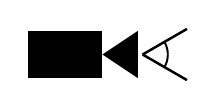
\begin{tikzpicture}[
  font=\sffamily\footnotesize,
]

% ---- 1. body rectangle (slightly longer than a square, black) ----
\pgfmathsetmacro{\bw}{0.95}      % body width
\pgfmathsetmacro{\bh}{0.60}      % body height (so ratio ~1.58 : 1)
\pgfmathsetmacro{\bxL}{0}
\pgfmathsetmacro{\bxR}{\bxL + \bw}
\pgfmathsetmacro{\byB}{0}
\pgfmathsetmacro{\byT}{\byB + \bh}
\pgfmathsetmacro{\bcy}{0.5*(\byB+\byT)}

\fill[black] (\bxL,\byB) rectangle (\bxR,\byT);

% ---- 2. triangle: tip at the rectangle, base on the right ----
\pgfmathsetmacro{\tlen}{0.45}    % how far the base sticks out to the right
\coordinate (triTip)  at (\bxR, \bcy);
\coordinate (triBaseT) at (\bxR + \tlen, \byT);
\coordinate (triBaseB) at (\bxR + \tlen, \byB);
\fill[black] (triTip) -- (triBaseT) -- (triBaseB) -- cycle;

% ---- 3. small gap then angle sign with arc ----
\pgfmathsetmacro{\gap}{0.06}
\pgfmathsetmacro{\angDeg}{30}     % half-FOV in degrees
\pgfmathsetmacro{\armLen}{0.65}
\pgfmathsetmacro{\arcR}{0.32}
\pgfmathsetmacro{\armX}{\armLen*cos(\angDeg)}
\pgfmathsetmacro{\armY}{\armLen*sin(\angDeg)}
\coordinate (angApex) at (\bxR + \tlen + \gap, \bcy);
\coordinate (angUp)   at ($(angApex) + (\armX,  \armY)$);
\coordinate (angDn)   at ($(angApex) + (\armX, -\armY)$);

\draw[black, line width=0.9pt] (angApex) -- (angUp);
\draw[black, line width=0.9pt] (angApex) -- (angDn);

% arc connecting the two arms close to the apex
\draw[black, line width=0.7pt]
  ($(angApex) + (\arcR, 0)$)
  arc (0:\angDeg:\arcR);
\draw[black, line width=0.7pt]
  ($(angApex) + (\arcR, 0)$)
  arc (0:-\angDeg:\arcR);

\end{tikzpicture}
\end{document}
